\documentclass{article}

\setlength{\parskip}{1em}
\setlength{\parindent}{0pt}

% Formatting and images 
\usepackage[utf8]{inputenc}
\usepackage[margin=1in]{geometry}
\usepackage[titletoc,title]{appendix}
\usepackage{authblk}
\usepackage{graphicx}
\usepackage{hyperref}
\usepackage{soul}
\usepackage{animate}


%% Language and font encodings
\usepackage[english]{babel}
\usepackage[T1]{fontenc}
\usepackage{booktabs}
\usepackage{indentfirst}
\usepackage{csquotes}
\nocite{*}

%% Packages for mathematical typesetting
\usepackage{amsmath}
\usepackage{amsthm}
\usepackage{amssymb}
\usepackage{gensymb}
\usepackage{pgf}
\usepackage{comment}
\usepackage{float}
\usepackage{blindtext}
\usepackage{enumitem}
\usepackage{bbm}
\usepackage{array}

%% Mathematical operators
\DeclareMathOperator*{\argmin}{arg\,min}

\newtheorem*{assumption}{Assumption}

\newtheorem{manualtheoreminner}{Theorem}
\newenvironment{manualtheorem}[1]{%
  \renewcommand\themanualtheoreminner{#1}%
  \manualtheoreminner
}{\endmanualtheoreminner}

% Title content
\title{\textbf{Title}}
\author[]{Henry Smith\\
Advised by Professor Harrison Zhou}
\affil[]{\normalsize Yale University}
\date{\today}

\begin{document}

% Title page
\maketitle

% Abstract
\begin{abstract}

\end{abstract}

\pagebreak

%Acknowledgment
\vspace*{\fill}

\begin{centering}
\section*{Acknowledgement}
\end{centering}

\vspace*{\fill}

\pagebreak
% Table of contents

\vspace*{\fill}

\begin{centering}
\tableofcontents
\end{centering}

\vspace*{\fill}

\pagebreak
% Begin content

\section{Overview}

\section{Preliminaries}\label{preliminaries}

The notation we present mirrors that of \cite{chizat2018lazy} and \cite{woodworth2020kernel}, since these two papers provide the main motivation for our research.

In particular, let $h: \mathbb{R}^P \rightarrow \mathcal{F}$ be a model mapping from parameter space $\mathbb{R}^p$ to Hilbert space $\mathcal{F}$. In the context of neural networks, we take $\mathcal{F}$ to be the Hilbert space consisting of all possible network functions. Then for each weight vector $\boldsymbol{w} \in \mathbb{R}^p$, our model $h$ specifies an associated network function $f \in \mathcal{F}$. More explicitly, we have the map $\boldsymbol{w} \mapsto f(\boldsymbol{w}, \cdot)$, where $f(\boldsymbol{w}, \cdot): \mathcal{X} \rightarrow \mathbb{R}$ is the neural network parameterized by weight vector $\boldsymbol{w}$. Here, $\mathcal{X}$ denotes the input space of the network $f$; for the purposes of our studies, we consider a Euclidean input space $\mathcal{X} \subseteq \mathbb{R}^n$. Of key importance in this notation is the distinction between $h$, which maps an individual weight vector to a network function, and $f(\boldsymbol{w}, \cdot)$, which maps an input point to a response value.

Since this notation is admittedly quite difficult to parse, we provide two illustrative examples which are of interest to our research. First, we consider the case in which $\mathcal{F} = \mathcal{X}^*$, the dual space of $\mathcal{X}$. Then for each weight vector $\boldsymbol{w} \in \mathbb{R}^p$, we get the corresponding network function $f(\boldsymbol{w}, \boldsymbol{x}) = \sum_{i=1}^n \boldsymbol{\tilde{w}}_i\boldsymbol{x}_i$ for some $\boldsymbol{\tilde{w}} \in \mathbb{R}^p$. That is, we associate with each weight vector a linear function in the input space $\mathcal{X}$. Let $(\boldsymbol{x}_1, y_1), \ldots, (\boldsymbol{x}_N, y_N)$ be the training points for our neural network, where each $\boldsymbol{x}_i \in \mathcal{X}$ and $y_i \in \mathbb{R}$. Moreover, let $\mathcal{D}$ be the empirical distribution determined by the training data $\{(\boldsymbol{x}_i, y_i) \}_{i=1}^N$. The keen reader will recognize that for $f(\boldsymbol{w}, \boldsymbol{x}) = \sum_{i=1}^n \boldsymbol{w}_i\boldsymbol{x}_i$, minimizing $\boldsymbol{w} \in \mathbb{R}^p$ with respect to the empirical risk, $\argmin_{\boldsymbol{w} \in \mathbb{R}^p} \  \mathbb{E}_{(\boldsymbol{x}, y) \sim \mathcal{D}}\left[\left(y - f(\boldsymbol{w}, \boldsymbol{x}) \right)^2 \right]$, is equivalent to simple linear regression. This linear regression example is that which is studied in \cite{woodworth2020kernel}. 

More generally, though, the network functions $f(\boldsymbol{w}, \cdot) \in \mathcal{F}$ need not be linear in the input space $\mathcal{X}$. And so to broaden our function class, we consider $\mathcal{F} = L^2(\mathcal{D}_{\boldsymbol{x}}, \mathcal{X})$, where $\mathcal{D}_{\boldsymbol{x}}$ is the $\boldsymbol{x}$ marginal distribution of $\mathcal{D}$ \cite{chizat2018lazy}. That is, we specify that for each vector $\boldsymbol{w} \in \mathbb{R}^p$, the corresponding network function $f(\boldsymbol{w}, \cdot)$ must be square integrable with respect to the distribution of input samples. If, in some hypothetical scenario, we were to know the population distribution of the input data $\mathcal{\rho_{\boldsymbol{x}}}$, we could instead take $\mathcal{F} = L^2(\rho_{\boldsymbol{x}}, \mathcal{X})$. Clearly, this is a broad function class $\mathcal{F}$ which encompasses many popular examples in contemporary deep learning.

Now that we have cleared up the meaning of $h$ and $f(\boldsymbol{w}, \cdot)$, we consider a certain property on $h$ which will be essential for our paper. In particular, we are interested in models $h$ which are \textit{$D$-positively homogeneous}. This means that for any $\boldsymbol{w} \in \mathbb{R}^p$ and any $\alpha \in \mathbb{R}_+$, $\alpha \neq 0$, then $h(\alpha \boldsymbol{w}) = \alpha^D h(\boldsymbol{w})$. Intuitively, $h$ $D$-positively homogeneous tells us that scaling the output of $h$ by a factor of $\alpha$ is equivalent to scaling the input by a factor of $\alpha^{1/D}$. The first example given above $h: \boldsymbol{w} \mapsto \sum_{i=1}^n \boldsymbol{w}_i \boldsymbol{x}_i$ provides an example of a 1-homogeneous model.

To conclude the setup of our paper, we consider how one would find an optimal weight vector $\boldsymbol{w}$ which minimizes some loss objective on $\mathcal{F}$. In particular, let $L: \mathcal{F} \rightarrow \mathbb{R}_+$ be the loss function mapping each element $f$ in our Hilbert space $\mathcal{F}$ to a nonnegative real number. An example of such a function $L$ is the mean-squared error or empirical risk 
\begin{align}
   L(f) = \mathbb{E}_{(\boldsymbol{x}, y) \sim \mathcal{D}} \left[ \left(y - f(\boldsymbol{x}) \right)^2 \right] = \frac{1}{N}\sum_{i=1}^N (y_i - f(\boldsymbol{x}_i))^2\label{mse}
\end{align}
that we mentioned above. 

Given a model $h: \mathbb{R}^p \rightarrow \mathcal{F}$ and corresponding loss function $L: \mathcal{F} \rightarrow \mathbb{R}_+$, we would like to use a gradient-based method to minimize the objective $L(h(\boldsymbol{w}))$. Surely, though, this would necessitate that we restrict our attention to $h$ and $L$ are everywhere differentiable on their domains. We formally state this assumption:
\begin{assumption}[from \cite{chizat2018lazy}]\label{assumption1}
The model $h: \mathbb{R}^p \rightarrow \mathcal{F}$ is differentiable with a locally Lipschitz differential $Dh$. Moreover, $L: \mathcal{F} \rightarrow \mathbb{R}_+$ is differentiable with a Lipschitz gradient.
\end{assumption}
As a consequence, we are able to define the \textit{gradient flow} dynamics on objective function $L(h(\boldsymbol{w}))$ with respect to $\boldsymbol{w} \in \mathbb{R}^p$. That is, we suppose that the network weights $\boldsymbol{w}(t)$ evolve in time $t \in \mathbb{R}_+$ according to the differential equation
\begin{align*}
    \boldsymbol{w}(t) = -\nabla L(\boldsymbol{w}(t)), \qquad \boldsymbol{w}(0) = \boldsymbol{w}_0
\end{align*}
where $\boldsymbol{w}_0 \in \mathbb{R}^p$ is some starting vector. Practitioners of deep learning should understand the gradient flow as a continuous time analogue to gradient descent \cite{wibisono2016}. Rather than choosing some positive stepsize with which we update our weights at $t \in \{0, 1, 2, \ldots \}$, gradient flow specifies the instantaneous direction in which we should update our weights at every time $t \in \mathbb{R}_+$.

\section{The Rich and Kernel Regimes, An Introduction}\label{richkernel}

\subsection{The Linearized Model}
As we detailed in the previous section, suppose we have some model $h: \mathbb{R}^p \rightarrow \mathcal{F}$ mapping a weight vector to a predictor function. And let $L: \mathcal{F} \rightarrow \mathbb{R}_+$ be a loss function which computes the misfit for each predictor function. Let $h$ and $L$ satisfy the differentiability assumption from Section \ref{preliminaries}. Moreover, suppose that our model $h$ is $D$-positively homogeneous. Using the gradient flow on the objective function $L(h(\boldsymbol{w}))$, we would like to find a $\boldsymbol{w}^{\star}$ such that $h(\boldsymbol{w}^{\star})$ minimizes $L$. Let us denote the gradient flow on $L(h(\boldsymbol{w}))$ by $(\boldsymbol{w}(t))_{t \geq 0}$ with starting point $\boldsymbol{w}(0) = \boldsymbol{w}_0$.

Corresponding to this model $h$, we have a \textit{linearized model} $\bar{h}$ defined
\begin{align}
    \bar{h}(\boldsymbol{w}) := h(\boldsymbol{w}_0) + Dh(\boldsymbol{w}_0)(\boldsymbol{w}-\boldsymbol{w}_0).\label{linearizedmodel}
\end{align}
In our particular case of $h(\boldsymbol{w}) = f(\boldsymbol{w}, \cdot)$ a neural network with $f(\boldsymbol{w}, \cdot): \mathcal{X} \rightarrow \mathbb{R}$, then we have
\begin{align}
    \bar{h}(\boldsymbol{w}) = \bar{f}(\boldsymbol{w}, \boldsymbol{x}) &=  f(\boldsymbol{w}_0, \boldsymbol{x}) + D_{\boldsymbol{w}}f(\boldsymbol{w}_0, \boldsymbol{x})(\boldsymbol{w}-\boldsymbol{w}_0) \nonumber\\ 
    &= f(\boldsymbol{w}_0, \boldsymbol{x}) + \langle \nabla_{\boldsymbol{w}} f(\boldsymbol{w}_0, \boldsymbol{x}), \boldsymbol{w}-\boldsymbol{w}_0\rangle, \quad \boldsymbol{x} \in \mathcal{X}.\label{linearizedmodelnetwork}
\end{align}

One will notice that the linearized model $\bar{h} = \bar{f}(\boldsymbol{w}, \cdot)$ is simply equal to the linearization of $h$ around its initialization $\boldsymbol{w}_0$ \cite{chizat2018lazy}. That is, $\bar{h}$ is an affine model in the weights $\boldsymbol{w}$ with $\bar{h}(\boldsymbol{w}_0) = h(\boldsymbol{w}_0) = f(\boldsymbol{w}_0, \boldsymbol{x})$ and $\nabla \bar{h}(\boldsymbol{w})|_{\boldsymbol{w} = \boldsymbol{\tilde{w}}} = \nabla h(\boldsymbol{w})|_{\boldsymbol{w} = \boldsymbol{w}_0} = \nabla_{\boldsymbol{w}} f(\boldsymbol{w}_0, \boldsymbol{x})$ for every $\boldsymbol{\tilde{w}} \in \mathbb{R}^p$. 

\subsection{Gradient Flow as a Kernel Method}\label{kernelmethod}

Now that we have presented the definition of the linearized model, let us analyze the special case of $h$ identically zero at its initialization $\boldsymbol{w}_0$ and loss $L$ the square loss, which is simply (\ref{mse}) scaled by a factor of $N$. Under these assumptions, the corresponding linearized model $\bar{h}$ is
\begin{align*}
    \bar{h}(\boldsymbol{w}) = \bar{f}(\boldsymbol{w}, \boldsymbol{x}) = \langle \nabla_{\boldsymbol{w}} f(\boldsymbol{w}_0, \boldsymbol{x}), \boldsymbol{w}-\boldsymbol{w}_0\rangle, \quad \boldsymbol{x} \in \mathcal{X}. 
\end{align*}
Let $(\boldsymbol{\bar{w}}(t))_{t \geq 0}$ be the gradient flow on $L(\bar{h}(\boldsymbol{w}))$ with $\boldsymbol{\bar{w}}(0) = \boldsymbol{w}_0$. We observe that for all times $t\in \mathbb{R}_+$, the predictor function $\bar{h}(\boldsymbol{\bar{w}}(t))$ can be expressed as $\langle \varphi(\boldsymbol{x}), \boldsymbol{\bar{w}}(t) - \boldsymbol{w}_0 \rangle$ for every $\boldsymbol{x} \in \mathcal{X}$, where $\varphi(\boldsymbol{x}) = \nabla_{\boldsymbol{w}} f(\boldsymbol{w}_0, \boldsymbol{x})$ and $\boldsymbol{w}(t) - \boldsymbol{w}_0 \in \mathbb{R}^p$. 

That is, for all times $t \in \mathbb{R}_+$, $\bar{h}(\boldsymbol{\bar{w}}(t))$ lies in the Reproducing Kernel Hilbert Space (RKHS) defined by the feature map $\varphi: \mathcal{X} \rightarrow \mathbb{R}^p$. The positive-definite kernel function $K: \mathcal{X} \times \mathcal{X} \rightarrow \mathbb{R}$ corresponding to this feature map $\varphi(\boldsymbol{x})$ is defined by
\begin{align}
    K(\boldsymbol{x}_1, \boldsymbol{x}_2) :&= \langle \varphi(\boldsymbol{x}_1), \varphi(\boldsymbol{x}_2) \rangle \nonumber \\
    &= \langle \nabla_{\boldsymbol{w}} f(\boldsymbol{w}_0, \boldsymbol{x}_1), \nabla_{\boldsymbol{w}} f(\boldsymbol{w}_0, \boldsymbol{x}_2) \rangle, \quad \forall \boldsymbol{x}_1, \boldsymbol{x}_2 \in \mathcal{X}\label{NTK}.
\end{align}

Therefore, finding a $\boldsymbol{w}^{\star} \in \mathbb{R}^p$ which minimizes $L(f(\boldsymbol{w}))$ is equivalent to finding a function $f^{\star}$ in the RKHS defined by feature map $\varphi$ which minimizes the square loss. More precisely stated, when $h(\boldsymbol{w}_0) = 0$ and $L$ is the square loss, then the gradient flow on $L(\bar{h}(\boldsymbol{w}))$ is equivalent to a kernel method with the \textit{neural tangent kernel} $K$ given by (\ref{NTK}) \cite{chizat2018lazy} \cite{jacot2018neural}.

\subsection{Relating the Nonlinear and Linearized Models}

So far, we have characterized the linearized model $\bar{h}$ corresponding to model $h$ and have justified that, under appropriate circumstances, gradient flow on the linearized objective $L(\bar{h}(\boldsymbol{w}))$ is equivalent to a kernel method. However, we have provided no reason to suggest that the original model $h$ should be at all similar to the linearized model $\bar{h}$: in general, even the most simple neural networks are highly nonlinear in their weights. 

Contrary to what one might expect, \cite{chizat2018lazy} rigorously argues that under certain conditions, the gradient flow on $L(h(\boldsymbol{w}))$, $(\boldsymbol{w}(t))_{t \geq 0}$, and that on $L(\bar{h}(\boldsymbol{w}))$, $(\boldsymbol{\bar{w}}(t))_{t \geq 0}$, remain close for all times $t \in \mathbb{R}_+$ with respect to the Euclidean norm $\| \cdot \|_p$. Furthermore, not only does \cite{chizat2018lazy} prove that $\boldsymbol{w}(t)$ and $\boldsymbol{\bar{w}}(t)$ are close, but also that the corresponding predictors $h(\boldsymbol{w}(t))$ and $h(\boldsymbol{\bar{w}}(t))$ are close with respect to $\| \cdot \|_{\mathcal{F}}$.

In order to fully understand this result and its implications, we must first define the scaled model $\alpha h(\boldsymbol{w})$ and the corresponding linearized model $\alpha \bar{h}(\boldsymbol{w})$ for $\alpha \in \mathbb{R}_+$, $\alpha \neq 0$. Corresponding to the scaled models, we define the scaled objective functions $\frac{1}{\alpha^2}L(\alpha h(\boldsymbol{w}))$ and $\frac{1}{\alpha^2}L(\alpha h(\boldsymbol{\bar{w}}))$. One should note that the multiplicative factor of $\frac{1}{\alpha^2}$ is no more than a positive scaling of the loss and does not affect the minimizer of either objective. Let $(\boldsymbol{w}_{\alpha}(t))_{t \geq 0}$ be the gradient flow on the objective $\frac{1}{\alpha^2}L(\alpha h(\boldsymbol{w}))$ and $(\boldsymbol{\bar{w}}_{\alpha}(t))_{t \geq 0}$ be the gradient flow on $\frac{1}{\alpha^2}L(\alpha \bar{h}(\boldsymbol{w}))$ satisfying $\boldsymbol{w}_{\alpha}(0) = \boldsymbol{\bar{w}}_{\alpha}(0) = \boldsymbol{w}_0$. And so all we have done is scale the output of our model $h$ by a factor of $\alpha$ and considered the gradient flow dynamics on the corresponding objective $\frac{1}{\alpha^2}L(\alpha h(\boldsymbol{w}))$.

Remarkably, Chizat and colleagues prove that, subject to certain conditions on the model $h$ and the loss $L$, as the scale of the output $\alpha \rightarrow \infty$, then training the model $\alpha h$ is equivalent to training the linearized model $\alpha \bar{h}$. The following two theorems summarize their results as they pertains to our research:

\begin{manualtheorem}{2.2}[from \cite{chizat2018lazy}]\label{Chizatthm2.2}
Assume that $h(\boldsymbol{w}_0) = 0$. Given a fixed time horizon $T > 0$, it holds that $\sup_{t \in [0, T]} \left\Vert \boldsymbol{w}_{\alpha}(t) - \boldsymbol{w}_0 \right\Vert = \mathcal{O}(1/\alpha)$,
\begin{align*}
    \sup_{t \in [0, T]} \left\Vert \boldsymbol{w}_{\alpha}(t) - \boldsymbol{\bar{w}}_{\alpha}(t) \right\Vert = \mathcal{O}(1/\alpha^2) \quad \text{and} \quad  \sup_{t \in [0, T]} \left\Vert \alpha h(\boldsymbol{w}_{\alpha}(t)) - \alpha \bar{h}(\boldsymbol{\bar{w}}_{\alpha}(t)) \right\Vert = \mathcal{O}(1/\alpha).
\end{align*}
\end{manualtheorem}

\begin{manualtheorem}{2.4}[from \cite{chizat2018lazy}]\label{Chizatthm2.4}
Consider the $M$-smooth and $m$-strongly convex loss $L$ with minimizer $f^{\star}$ and condition number $\kappa := M/m$. Assume that $\sigma_{\text{min}}$, the smallest singular value of $Dh(\boldsymbol{w}_0)^T$, is positive and that the initialization satisfies $\left\Vert h(\boldsymbol{w}_0) \right\Vert \leq C_0:= \sigma_{\text{min}}^3/(32\kappa^{3/2} \left\Vert Dh(\boldsymbol{w}_0) \right\Vert \text{Lip}(Dh))$, where $\text{Lip}(Dh)$ is the Lipschitz constant of $Dh$. If $\alpha > \left\Vert f^{\star} \right\Vert / C_0$, then for $t \in \mathbb{R}_+$, it holds
\begin{align*}
    \left\Vert \alpha h(\boldsymbol{w}_{\alpha}(t)) - y^{\star} \right\Vert \leq \sqrt{\kappa} \left\Vert \alpha h(\boldsymbol{w}_0) - f^{\star} \right\Vert \exp( -m \sigma_{\text{min}}^2 t/4).
\end{align*}
If moreover $h(\boldsymbol{w}_0) = 0$, it holds as $\alpha \rightarrow \infty$, $\sup_{t \geq 0} \left\Vert \boldsymbol{w}_{\alpha}(t) - \boldsymbol{w}_0 \right\Vert = \mathcal{O}(1/\alpha)$,
\begin{align*}
    \sup_{t \geq 0} \left\Vert \alpha h(\boldsymbol{w}_{\alpha}(t)) - \alpha \overline{h}(\boldsymbol{\bar{w}}_{\alpha}(t)) \right\Vert = \mathcal{O}(1/\alpha) \quad \text{and} \quad  \sup_{t \geq 0} \left\Vert \boldsymbol{w}_{\alpha}(t) - \boldsymbol{\bar{w}}_{\alpha}(t) \right\Vert = \mathcal{O}(\log \alpha/\alpha^2).
\end{align*}
\end{manualtheorem}

Starting with Theorem \ref{Chizatthm2.2}, we have that for model $h$ satisfying $h(\boldsymbol{w}_0) = 0$ and fixed time $T > 0$, the $\ell^p$ distance between $\boldsymbol{w}_{\alpha}(t)$, the gradient flow path of $\frac{1}{\alpha^2} L(\alpha h(\boldsymbol{w}))$, and $\boldsymbol{w}_0$, the initialization of the gradient flow, for $t \in [0, T]$ is no greater than $\mathcal{O}(1/\alpha)$. This is a result that we had not previously discussed: in the limit as $\alpha \rightarrow \infty$, the weights $\boldsymbol{w}_{\alpha}(t)$ of the network $f(\boldsymbol{w}_{\alpha}(t), \boldsymbol{x})$ remain constant throughout training on any finite interval $[0, T]$, $T > 0$. Moreover, as we had previously hinted at, the distance between the gradient flow path of the scaled original model, $\boldsymbol{w}_{\alpha}(t)$, and that of the scaled linearized model, $\boldsymbol{\bar{w}}_{\alpha}(t)$, is no greater than $\mathcal{O}(1/\alpha^2)$ for any $t \in [0, T]$. Looking at the networks $\alpha h(\boldsymbol{w}_{\alpha}(t)), \alpha h(\boldsymbol{\bar{w}}_{\alpha}(t)) \in \mathcal{F}$ themselves, Theorem \ref{Chizatthm2.2} also gives us that the distance between $\alpha h(\boldsymbol{w}_{\alpha}(t))$ and $\alpha h(\boldsymbol{\bar{w}}_{\alpha}(t))$ in the Hilbert space norm is no greater than $\mathcal{O}(1/\alpha)$ for each $t \in [0, T]$.

Although Theorem \ref{Chizatthm2.2} is certainly valuable insofar that it characterizes the gradient flow dynamics on $\frac{1}{\alpha^2}L(\alpha h(\boldsymbol{w}))$ and $\frac{1}{\alpha^2}L(\alpha \bar{h}(\boldsymbol{w}))$ for each finite time horizon $T > 0$, it does not provide us a bound that is uniform in $t \in \mathbb{R}_+$. A uniform bound is of particular importance if we would like to say something about the solutions (i.e. networks) reached by the gradient flow on the two scaled objective functions. In order to get such a bound, we must appeal to Theorem \ref{Chizatthm2.4}, which makes stronger assumptions on the loss function $L$ and the derivative of the model $h$, $Dh$. In particular, we require that our loss function is both convex as well as $M$-smooth, $m$-strongly convex. An example of such a loss is the mean-squared error or empirical risk (\ref{mse}). Furthermore, we need it to be the true that the derivative of $h$ is surjective. As noted in \cite{chizat2018lazy}, this can only be the case if the Hilbert space $\mathcal{F}$ is finite-dimensional, such as for $\mathcal{F} = \mathcal{X}^*$.

One will notice that Theorem \ref{Chizatthm2.4} expands the results in Theorem \ref{Chizatthm2.2} to be independent of time $t \in \mathbb{R}_+$, giving us the uniform bounds in $t$ that we desired. This tells us that in the $\alpha \rightarrow \infty$ limit, the gradient flow on the scaled original objective is exactly equivalent to that on the scaled linearized objective. Not only are the solutions reached by $(\boldsymbol{w}_{\alpha}(t))_{t \geq 0}$ and $(\boldsymbol{\bar{w}}_{\alpha}(t))_{t \geq 0}$ the same, but so are gradient flow paths themselves (i.e. $\boldsymbol{w}_{\alpha}(t) \rightarrow \boldsymbol{\bar{w}}_{\alpha}(t)$ as $\alpha \rightarrow \infty$ for every $t \in \mathbb{R}_+$). Just as important, Theorem \ref{Chizatthm2.4} also states that in the limit $\alpha \rightarrow \infty$, the gradient flow on $\frac{1}{\alpha^2}L(\alpha h(\boldsymbol{w}))$ converges exponentially to a global minimizer $f^{\star}$ of the loss $L$. This convergence gaurantee is a powerful result since the objective $L(h(\boldsymbol{w}))$ is not a priori convex in $\boldsymbol{w} \in \mathbb{R}^p$, and so we are solving a nonconvex optimization problem.

Recall our assumption that $h$ is $D$-positively homogeneous, and so $\alpha h(\boldsymbol{w}) = h(\alpha^{1/D}\boldsymbol{w})$ as well as $\alpha \bar{h}(\boldsymbol{w}) = \bar{h}(\alpha^{1/D}\boldsymbol{w})$.
Therefore, the gradient flow on the scaled objective $\frac{1}{\alpha^2}L(\alpha h(\boldsymbol{w}))$ with initialization $\boldsymbol{w}_{\alpha}(0) = \boldsymbol{w}_0$ is exactly the same as the gradient flow on the unscaled objective $\frac{1}{\alpha^2}L(h(\boldsymbol{w}))$ with initialization $\boldsymbol{w}_{\alpha}(0) = \alpha^{1/D}\boldsymbol{w}_0$. Throughout the remainder of the paper, we will consider the second scenario in which the initialization $\boldsymbol{w}_0$ is scaled by $\alpha$ as opposed to the model output $h(\boldsymbol{w}_{\alpha}(t))$. 

\subsection{Defining the Kernel and Rich Regimes}

Altogether, Theorems \ref{Chizatthm2.2} and \ref{Chizatthm2.4} from \cite{chizat2018lazy} formulate the \textit{kernel limit} that will be of primary interest in Sections \ref{summarizekernel} and \ref{summarizekernel}. To conclude this portion of our paper, we make clear our definition of the kernel limit and contrast it with the \textit{rich limit}. 

To be explicit, the kernel limit occurs when the initialization scale $\alpha \in \mathbb{R}_+$, $\alpha \neq 0$ of the gradient flow $(\boldsymbol{w}_{\alpha}(t))_{t \geq 0}$, $\boldsymbol{w}_{\alpha}(0) = \alpha \boldsymbol{w}_0$ on objective $\frac{1}{\alpha^2}L(h(\boldsymbol{w}))$ tends to infinity for the $D$-homogeneous model $h$ satisfying $h(\boldsymbol{w}_0) = 0$. From the work of Chizat and colleagues we know that, under certain conditions on $h$ and $L$, training the nonlinear model $h$ with gradient flow is equivalent to training the affine model $\bar{h}$ as $\alpha \rightarrow \infty$. This is how the kernel limit gets its name: in the limit $\alpha \rightarrow \infty$, training $h$ with the square loss $L$ is equivalent to a kernel method with the neural tangent kernel $K$ (see Section \ref{kernelmethod}). As we mentioned in our discussion of Theorem \ref{Chizatthm2.2}, the kernel limit is equivalently characterized by the distance of the gradient flow from its initialization $\alpha \boldsymbol{w}_0$. In particular, as $\alpha \rightarrow \infty$, the network weights become constant throughout training. It is for this reason that Chizat and colleagues refer to the kernel limit as \enquote{lazy training.} 

Note that in practice, we will never observe the true kernel limit $\alpha \rightarrow \infty$. Therefore, we use the term \textit{kernel regime} to refer to the approximation of the kernel limit: when $\boldsymbol{w}_{\alpha}(t)$ is close to $\boldsymbol{\bar{w}}_{\alpha}(t)$ and $h(\boldsymbol{w}_{\alpha}(t))$ is close to $h(\boldsymbol{\bar{w}}_{\alpha}(t))$ in their respective norms for all times $t \geq 0$.

As evidenced by the contemporary field of deep learning, the models that we wish to optimize are often highly nonlinear in $\boldsymbol{w}$ around their initialization $\alpha\boldsymbol{w}_0$, and so the gradient flow on $\frac{1}{\alpha^2}L(h(\boldsymbol{w}))$ does not operate in the kernel regime. That is, the difference between $\boldsymbol{w}_{\alpha}(t)$ and $\boldsymbol{\bar{w}}_{\alpha}(t)$ as well as the difference between $h(\boldsymbol{w}_{\alpha}(t))$ and $h(\boldsymbol{\bar{w}}_{\alpha}(t))$ are large for all times $t \in \mathbb{R}_+$. We refer to this phenomenon as the \textit{rich regime} which corresponds to the \textit{rich limit} $\alpha \rightarrow 0$. Analogous to the kernel limit, the rich limit can be equivalently described in terms of the distance between the gradient flow path $\boldsymbol{w}_{\alpha}(t)$ and the gradient flow initialization $\alpha\boldsymbol{w}_0$. In the rich limit, $\boldsymbol{w}_{\alpha}(t)$ moves far from its initialization $\boldsymbol{w}_{\alpha}(0) = \alpha \boldsymbol{w}_0$ during training. As a result, Woodworth and colleagues refer to the rich limit as \enquote{active training,} matching the title given to the kernel limit by Chizat and colleagues.

The distinction between the kernel and rich regimes is important because gradient flow in each regime leads to distinct \textit{implicit biases} in the resulting model $h(\lim_{t \to\infty} \boldsymbol{w}_{\alpha}(t))$. In other words, the solution to the gradient flow on $\frac{1}{\alpha^2}L(h(\boldsymbol{w}))$ will result in a network $h(\lim_{t \to\infty} \boldsymbol{w}_{\alpha}(t)) = f(\lim_{t \to\infty} \boldsymbol{w}_{\alpha}(t), \boldsymbol{x}), \ \boldsymbol{x} \in \mathcal{X}$ that has different properties depending on whether gradient flow operated in the kernel or rich regime. As we will more thoroughly examine in Sections \ref{summarizekernel} and \ref{summarizekernel}, the most influential hypothesis made by Woodworth and colleagues in \cite{woodworth2020kernel} is that training a network in the rich regime implicitly imposes sparsity on its parameters, which is not the case for the kernel regime. If true, this would allow for better generalization in certain sparse problems (i.e. the underlying model from which the data $(\boldsymbol{x}, y)$ is generated is sparse) when the network is trained in the rich regime as opposed to the kernel regime.

\section{Visualizing the Kernel Regime}\label{summarizekernel}

In Section \ref{richkernel}, we rigorously defined the kernel and rich regimes for a $D$-homogeneous model $h: \mathbb{R}^p \rightarrow \mathcal{F}$ and loss function $L: \mathcal{F} \rightarrow \mathbb{R}_+$ satisfying some differentiability conditions. However, our discussion of the kernel and rich regimes has so far been purely theoretical. In this section, we seek to empirically demonstrate that the results from \cite{chizat2018lazy} do, in fact, hold. In order to do so, we focus our attention on the simple linear regression problem studied by Woodworth and colleagues in \cite{woodworth2020kernel}. Although the model under consideration is the same, the code, experiments, and visualizations we present are of our own formulation.

\subsection{Simple Linear Regression}

To begin, we introduce the simple linear regression model from \cite{woodworth2020kernel} with which we will demonstrate the kernel and rich regimes.

Consider a set of training data $\{ (\boldsymbol{x}_i, y_i)\}_{i=1}^N$, where each $\boldsymbol{x}_i \in \mathcal{X} = \mathbb{R}^n$ and $y_i \in \mathbb{R}$ for $1 \leq i \leq N$. Then, corresponding to this training dataset, we specify the linear regression model $h: \mathbb{R}^{2n} \rightarrow (\mathbb{R}^n)^*$ such that
\begin{align}\label{linreg}
    h(\boldsymbol{w}) = f(\boldsymbol{w}, \boldsymbol{x}) = \sum_{i=1}^n(\boldsymbol{w}_{+, i}^2 - \boldsymbol{w}_{-, i}^2)\boldsymbol{x}_i \quad 
    \boldsymbol{w} = 
    \begin{bmatrix}
        \boldsymbol{w}_+ \\
        \boldsymbol{w}_-
    \end{bmatrix} 
    \in \mathbb{R}^{2n} \quad \boldsymbol{x} \in \mathcal{X}.
\end{align}
It may appear odd that we have parameterized the linear regression model in this way. Namely, why do we have two sets of weights $\boldsymbol{w}_{+, i}$ and $\boldsymbol{w}_{-, i}$ corresponding to each input dimension, and why are the individual weights squared? As is discussed in \cite{woodworth2020kernel}, the two sets of weights ensure that the image of $h$ is all of $(\mathbb{R}^n)^*$, the Hilbert space of linear functionals on $\mathbb{R}^n$. If this were not the case, then we would have linear regression with the additional constraint that all the coefficients need be positive. The individual components of the weight vector $\boldsymbol{w}$ are squared so that the model $h$ is two-positively homogeneous: $\sum_{i=1}^n((\alpha \boldsymbol{w}_{+, i})^2 - (\alpha \boldsymbol{w}_{-, i})^2)\boldsymbol{x}_i = \alpha^2\sum_{i=1}^n(\boldsymbol{w}_{+, i}^2 - \boldsymbol{w}_{-, i}^2)\boldsymbol{x}_i$ for each $\alpha \in \mathbb{R}_+$, $\alpha \neq 0$.

Further, our linear regression model $f(\boldsymbol{w}, \boldsymbol{x})$ is linear in the input space $\mathcal{X}$. Therefore, as is guaranteed by the Riesz-Representation Theorem, we can express $h(\boldsymbol{w})$ as 
\begin{align}
    h(\boldsymbol{w}) = f(\boldsymbol{w}, \boldsymbol{x}) = \langle \boldsymbol{\beta}_{\boldsymbol{w}}, \boldsymbol{x} \rangle, \quad \boldsymbol{\beta}_{\boldsymbol{w}} = \boldsymbol{w}_{+}^2 - \boldsymbol{w}_{i}^2, \quad \boldsymbol{x} \in \mathcal{X},
\end{align}
where $\boldsymbol{z}^2$ denotes element-wise squaring of the vector $\boldsymbol{z} \in \mathbb{R}^n$. If it was not already clear, one should observe that the vector $\boldsymbol{\beta}_{\boldsymbol{w}}$ is the classical linear regression coefficient vector. Also, we mention that whenever $\boldsymbol{w}$ satisfies $\boldsymbol{w}_+ = \boldsymbol{w}_-$, then $h(\boldsymbol{w}) = \langle \boldsymbol{\beta}_{\boldsymbol{w}}, \boldsymbol{x} \rangle = \langle \boldsymbol{0}, \boldsymbol{x} \rangle = 0$.

As for our loss function $L: (\mathbb{R}^n)^* \rightarrow \mathbb{R}_+$, we will work with the mean-squared error (\ref{mse}). This differs from the square loss considered in \cite{woodworth2020kernel} only by a factor of $\frac{1}{N}$, and so the set of minimizers of the two losses is identical.

Having described both the linear regression model $h$ as well as the mean-squared error $L$, we state an additional assumption that is important for investigating the problem:
\begin{assumption}
Let $N \leq n$, meaning the dimension of the input space is at least as large as the number of training points.
\end{assumption}
We make this assumption because, as previously discussed, we are interested in the different solutions to the gradient flow dynamics when trained in the kernel and rich regimes. Taking $N \leq n$ ensures that the system $\boldsymbol{X}\boldsymbol{\beta}_{\boldsymbol{w}} = \boldsymbol{y}$ is underdetermined, and so there are usually (but not always), many solutions for $\boldsymbol{\beta}_{\boldsymbol{w}}$. Equivalently stated, we choose our network $f(\boldsymbol{w}, \boldsymbol{x})$ to be overparameterized so that there are many potential weight vectors $\boldsymbol{w}$ which minimize the objective $L(h(\boldsymbol{w}))$.

\subsubsection{Explicit Solutions for the Kernel and Rich Limits}
Albeit quite straightforward and lacking in complexity, the linear regression problem is well-suited for studying the implicit biases resulting from training in the kernel and rich regimes. Woodworth and colleagues provide a thorough characterization of these implicit biases, which we summarize in the remainder of this section. In particular, let us consider the gradient flow on $L(h(\boldsymbol{w}))$, $(\boldsymbol{w}_{\alpha}(t))_{t \geq 0}$, with initialization $\boldsymbol{w}_{\alpha}(0) = \alpha \mathbbm{1}$. That is, we are looking at the gradient flow on the objective with initialization scaled by a factor of $\alpha \in \mathbb{R}_+$, $\alpha \neq 0$. Also, we are explicitly choosing $\boldsymbol{w}_0 = \mathbbm{1}$ so that $h(\boldsymbol{w}_0) = 0$, as we pointed out above.

First, let us determine the kernel limit. Writing down the feature map $\varphi(\boldsymbol{x}) = \nabla_{\boldsymbol{w}} f(\boldsymbol{w}_{\alpha}(0), \boldsymbol{x})$ explicitly, 
\begin{align*}
    \varphi(\boldsymbol{x}) &= \nabla_{\boldsymbol{w}}\left( \sum_{i=1}^n(\boldsymbol{w}_{+, i}^2 - \boldsymbol{w}_{-, i}^2)\boldsymbol{x}_i \right)\bigg|_{\boldsymbol{w} = \boldsymbol{w}_{\alpha}(0)}\\
    &= 
    2\begin{bmatrix}
        (\boldsymbol{w}_+) \odot \boldsymbol{x}\\
        -(\boldsymbol{w}_-) \odot \boldsymbol{x}
    \end{bmatrix} \bigg|_{\boldsymbol{w} = \boldsymbol{w}_{\alpha}(0)}\\
    &= 2\alpha \begin{bmatrix}
        \boldsymbol{x}\\
        -\boldsymbol{x}
    \end{bmatrix}.
\end{align*}
Here, $\boldsymbol{y} \odot \boldsymbol{z}$ denotes the element-wise product of vectors $\boldsymbol{y}, \boldsymbol{z} \in \mathbb{R}^n$. From \cite{woodworth2020kernel}, we know that for the square loss $\tilde{L}$, the $\boldsymbol{w}^{\star} = \lim_{t \to \infty} \boldsymbol{\bar{w}}_{\alpha}(t)$ reached by gradient flow on the objective $\tilde{L}(\bar{h}(\boldsymbol{w}))$ satisfies $\bar{h}(\boldsymbol{w}^{\star}) = \argmin_{f \in (\mathbb{R}^n)^*} \| f \|_{K}, \ f(\boldsymbol{X}) = \boldsymbol{y}$, where $\| \cdot \|_K$ is the RKHS norm determined by $\varphi(\boldsymbol{x})$. And by Theorem \ref{Chizatthm2.4}, we know that it is indeed the case that the resulting predictor function $\bar{h}(\boldsymbol{w}^{\star})$ is a global minimizer of the loss $L$ \cite{chizat2018lazy}. Expanding out the definition of the RKHS norm, we get:
\begin{align}
    \bar{h}(\boldsymbol{w}^{\star}) &= \argmin_{f \in (\mathbb{R}^n)^*} \| f \|_{K}, \quad f(\boldsymbol{X}) = \boldsymbol{y} \nonumber\\
    &= \argmin_{f \in (\mathbb{R}^n)^*} \left( \inf \left\{ \| \boldsymbol{w} \|_2 : \boldsymbol{w} \in \mathbb{R}^{2n},  f(\boldsymbol{x}) = \langle \boldsymbol{w}, \varphi(\boldsymbol{x}) \rangle, \ \forall \boldsymbol{x} \in \mathcal{X} \right\}\right), \quad f(\boldsymbol{X}) = \boldsymbol{y} \nonumber\\
    &= \argmin_{f \in (\mathbb{R}^n)^*} \left( \inf \left\{ \| \boldsymbol{w} \|_2 : \boldsymbol{w} \in \mathbb{R}^{2n},  f(\boldsymbol{x}) = 2\alpha \langle \boldsymbol{w}_+ - \boldsymbol{w}_-, \boldsymbol{x} \rangle, \ \forall \boldsymbol{x} \in \mathcal{X} \right\}\right), \quad f(\boldsymbol{X}) = \boldsymbol{y} \nonumber\\
    &= \argmin_{f \in (\mathbb{R}^n)^*} \left( \inf \left\{ \| \boldsymbol{w} \|_2 : \boldsymbol{w} \in \mathbb{R}^{2n},  f(\boldsymbol{x}) = \langle \boldsymbol{w}_+ - \boldsymbol{w}_-, \boldsymbol{x} \rangle, \ \forall \boldsymbol{x} \in \mathcal{X} \right\}\right), \quad f(\boldsymbol{X}) = \boldsymbol{y}.\label{RKHSnorm}
\end{align}
Since $f \in (\mathbb{R}^n)^* \Leftrightarrow f(\boldsymbol{x}) = \langle \boldsymbol{\beta}, \boldsymbol{x} \rangle, \ \forall \boldsymbol{x} \in \mathcal{X}$ for some $\boldsymbol{\beta} \in \mathbb{R}^n$, then (\ref{RKHSnorm}) implies that $\bar{h}(\boldsymbol{w}^{\star}) = f(\boldsymbol{w}^{\star}, \boldsymbol{x}) =  \langle \boldsymbol{\beta}_{\boldsymbol{w}}^{\star}, \boldsymbol{x} \rangle \ \forall \boldsymbol{x} \in \mathcal{X}$, where $\boldsymbol{\beta}_{\boldsymbol{w}}^{\star}$ satisfies
\begin{align*}
    \boldsymbol{\beta}_{\boldsymbol{w}}^{\star} &= \argmin_{\boldsymbol{\beta} \in \mathbb{R}^n} \left( \inf \left\{ \| \boldsymbol{w} \|_2 : \boldsymbol{w} \in \mathbb{R}^{2n},  \boldsymbol{\beta} = \boldsymbol{w}_+ - \boldsymbol{w}_- \right\}\right), \quad \boldsymbol{X}\boldsymbol{\beta} = \boldsymbol{y}\\
    &= \argmin_{\boldsymbol{\beta} \in \mathbb{R}^n} \| \boldsymbol{\beta} \|_2, \quad \boldsymbol{X}\boldsymbol{\beta} = \boldsymbol{y}.
\end{align*}
To summarize, the solution $\boldsymbol{w}^{\star}$ to the gradient flow dynamics $(\boldsymbol{w}_{\alpha}(t))_{t \geq 0}$, $\boldsymbol{w}(0) = \alpha \mathbbm{1}$ on $L(h(\boldsymbol{w}))$ in the kernel limit $\alpha \rightarrow \infty$ satisfies $h(\boldsymbol{w}^{\star}) =\langle \boldsymbol{\beta}_{\ell^2}, \boldsymbol{x} \rangle, \ \forall \boldsymbol{x} \in \mathcal{X}$, where $\boldsymbol{\beta}_{\ell^2} \in \mathbb{R}^n$ is the minimum $\ell^2$ solution to $\boldsymbol{X} \boldsymbol{\beta} = \boldsymbol{y}$. We are able to refer to $(\boldsymbol{w}_{\alpha}(t))_{t \geq 0}$ and $(\boldsymbol{\bar{w}}_{\alpha}(t))_{t \geq 0}$ as well as $h$ and $\bar{h}$ interchangeably since we are operating in the kernel limit $\alpha \rightarrow \infty$.

In order to treat the rich limit, we rely on a result from Gunasekar and colleagues. In particular, \cite{gunasekar2018implicit} considers the matrix factorization problem $\langle \boldsymbol{A}_i, \boldsymbol{Z} \rangle = y_i$, where $\{ \boldsymbol{A}_i \}_{i=1}^N$ are commutative measurement matrices, $\{ y_i \}_{i=1}^N$ are output values, and $\boldsymbol{Z}$ is some unknown matrix. The authors take the loss $\tilde{L}$  to be the square loss $\sum_{i=1}^N (y_i - \langle \boldsymbol{A}_i, \boldsymbol{Z} \rangle)^2$ and define the gradient flow $(\boldsymbol{Z}_{\alpha}(t))_{t \geq 0}$, $\boldsymbol{Z}_{\alpha}(0) = \alpha \boldsymbol{Z}_0$ on the objective $\tilde{L}(\mathcal{A}(\boldsymbol{Z}))$. Here, $\mathcal{A}(\boldsymbol{Z}) \in \mathbb{R}^n$ is the prediction vector defined $\mathcal{A}(\boldsymbol{Z})_i = \langle \boldsymbol{A}_i, \boldsymbol{Z} \rangle$. 

While, at first glance, the linear regression problem at hand seems seems unrelated to matrix factorization, we remark that it is, in fact, a special case. To see why this is true, suppose that we take each $\boldsymbol{A}_i$ to be a diagonal matrix $(\boldsymbol{A}_i)_{j,j} = (\boldsymbol{x}_i)_j$, $1 \leq j \leq n$ corresponding to the $i$th training observation in the linear regression data. Moreover, let us choose our initial matrix $\boldsymbol{Z}_0$ for gradient flow to be $\mathbbm{I}_{n \times n}$. Then for all times $t \in \mathbb{R}_+$, $\boldsymbol{Z}_{\alpha}(t)$ will be a diagonal matrix with $\langle \boldsymbol{A}_i, \boldsymbol{Z}_{\alpha}(t) \rangle = \langle \boldsymbol{\beta}_{\boldsymbol{w}},\boldsymbol{x}_i \rangle$ for each $1 \leq i \leq N$, where $\boldsymbol{\beta}_{\boldsymbol{w}} \in \mathbb{R}^n$, $(\boldsymbol{\beta}_{\boldsymbol{w}})_j = (\boldsymbol{Z}_{\alpha}(t))_{j,j}$ is the vector containing the diagonal entries of $\boldsymbol{Z}_{\alpha}(t)$. From here, we see that this particular instance of the matrix factorization problem ($\boldsymbol{A}_i$ diagonal matrices, $\boldsymbol{Z}_0$ a diagonal matrix) is simply an alternate parameterization of simple linear regression.

Now that we have justified looking at the matrix factorization problem, let us state the following result proven by Gunasekar and colleagues:
\begin{manualtheorem}{1}[from \cite{gunasekar2018implicit}]
In the case where the matrices $\{\boldsymbol{A}_i\}_{i=1}^m$ commute, if $\boldsymbol{Z}_0^{\star} = \lim_{\alpha \rightarrow 0} \boldsymbol{Z}_{\alpha}^{\star}$ exists and is a global optima for the matrix factorization problem with $\mathcal{A}(\boldsymbol{Z}_0^{\star}) = y$, then $\boldsymbol{Z}_0^{\star} \in \argmin_{\boldsymbol{Z} \succeq 0} \|\boldsymbol{Z} \|_* \\ \ \text{s.t.} \ \mathcal{A}(\boldsymbol{Z}) = \boldsymbol{y}$. Here, $\boldsymbol{Z}_{\alpha}^{\star}$ is the solution $\lim_{t \to \infty} \boldsymbol{Z}_{\alpha}(t)$ to the gradient flow $(\boldsymbol{Z}_{\alpha}(t))_{t \geq 0}$, $\boldsymbol{Z}_{\alpha}(0) = \alpha \boldsymbol{Z}_0$.
\end{manualtheorem}
In the case of our linear regression problem, the matrix $\boldsymbol{Z}$ is diagonal, and so the nuclear norm is equal to the $\ell^1$ norm. This means that
\begin{align*}
    \boldsymbol{Z}_0^{\star} \in \argmin_{\boldsymbol{Z} \succeq 0} \|\boldsymbol{Z} \|_* \ \mathcal{A}(\boldsymbol{Z}) = \boldsymbol{y} \quad  \Longleftrightarrow \quad \boldsymbol{\beta}_{\boldsymbol{w}} \in \argmin_{\boldsymbol{\beta} \in \mathbb{R}_+^n} \| \boldsymbol{\beta} \|_1 \ \boldsymbol{X} \boldsymbol{\beta} = \boldsymbol{y}.
\end{align*}
That is, the solution $\boldsymbol{w}^{\star}$ to the gradient flow $(\boldsymbol{w}_{\alpha}(t))_{t \geq 0}$, $\boldsymbol{w}(0) = \alpha \mathbbm{1}$ on $L(h(\boldsymbol{w}))$ in the rich limit $\alpha \rightarrow 0$ satisfies $h(\boldsymbol{w}^{\star}) = \langle \boldsymbol{\beta}_{\ell^1}, \boldsymbol{x} \rangle, \ \forall \boldsymbol{x} \in \mathcal{X}$, where $\boldsymbol{\beta}_{\ell^1}$ is the minimum $\ell^1$ solution to $\boldsymbol{X} \boldsymbol{\beta} = \boldsymbol{y}$, $\boldsymbol{\beta} \in \mathbb{R}_+^n$. If the minimum $\ell^1$ solution to $\boldsymbol{X} \boldsymbol{\beta} = \boldsymbol{y}$ is contained in $\mathbb{R}_+^n$, then $\boldsymbol{\beta}_{\ell^1} = \argmin_{\beta \in \mathbb{R}^n} \| \boldsymbol{\beta} \|, \ \boldsymbol{X} \boldsymbol{\beta} = \boldsymbol{y}$ (i.e. $\boldsymbol{\beta}_{\ell^1}$ is the true $\ell^1$ solution to the system $\boldsymbol{X} \boldsymbol{\beta} = \boldsymbol{y}$).

And so we have written down explicit formulas both for the kernel and rich limits corresponding to the simple linear regression problem $h(\boldsymbol{w}) = f(\boldsymbol{w}, \boldsymbol{x}) = \sum_{i=1}^n(\boldsymbol{w}_{+, i}^2 - \boldsymbol{w}_{-, i}^2)\boldsymbol{x}_i = \langle \boldsymbol{\beta}_{\boldsymbol{w}}, \boldsymbol{x} \rangle $ with loss $L$ the mean-squared error. The result we have presented is particularly salient as it gives a clear characterization of the implicit biases that result from training in the kernel and rich regimes. In particular, under appropriate conditions on the system $\boldsymbol{X} \boldsymbol{\beta} = \boldsymbol{y}$, the solution to the gradient flow dynamics in the kernel limit is the minimum $\ell^2$ solution $\boldsymbol{\beta}_{\ell^2}$, whereas the the solution in the rich limit is the minimum $\ell^2$ solution $\boldsymbol{\beta}_{\ell^1}$. Woodworth and colleagues go even a step further and indicate how the gradient flow solution interpolates between the minimum $\ell^1$ and $\ell^2 $ solutions as the initialization scale $\alpha$ interpolates between $0$ and $\infty$ (see Theorem 1 in \cite{woodworth2020kernel}). The consequences of this result are self-evident: in the linear regression setting, one can choose their initialization scale $\alpha$ carefully in order to achieve either $\ell^1$ or $\ell^2$ shrinkage.

\subsection{The Linearized Model}

\begin{figure}[H]
    \centering
    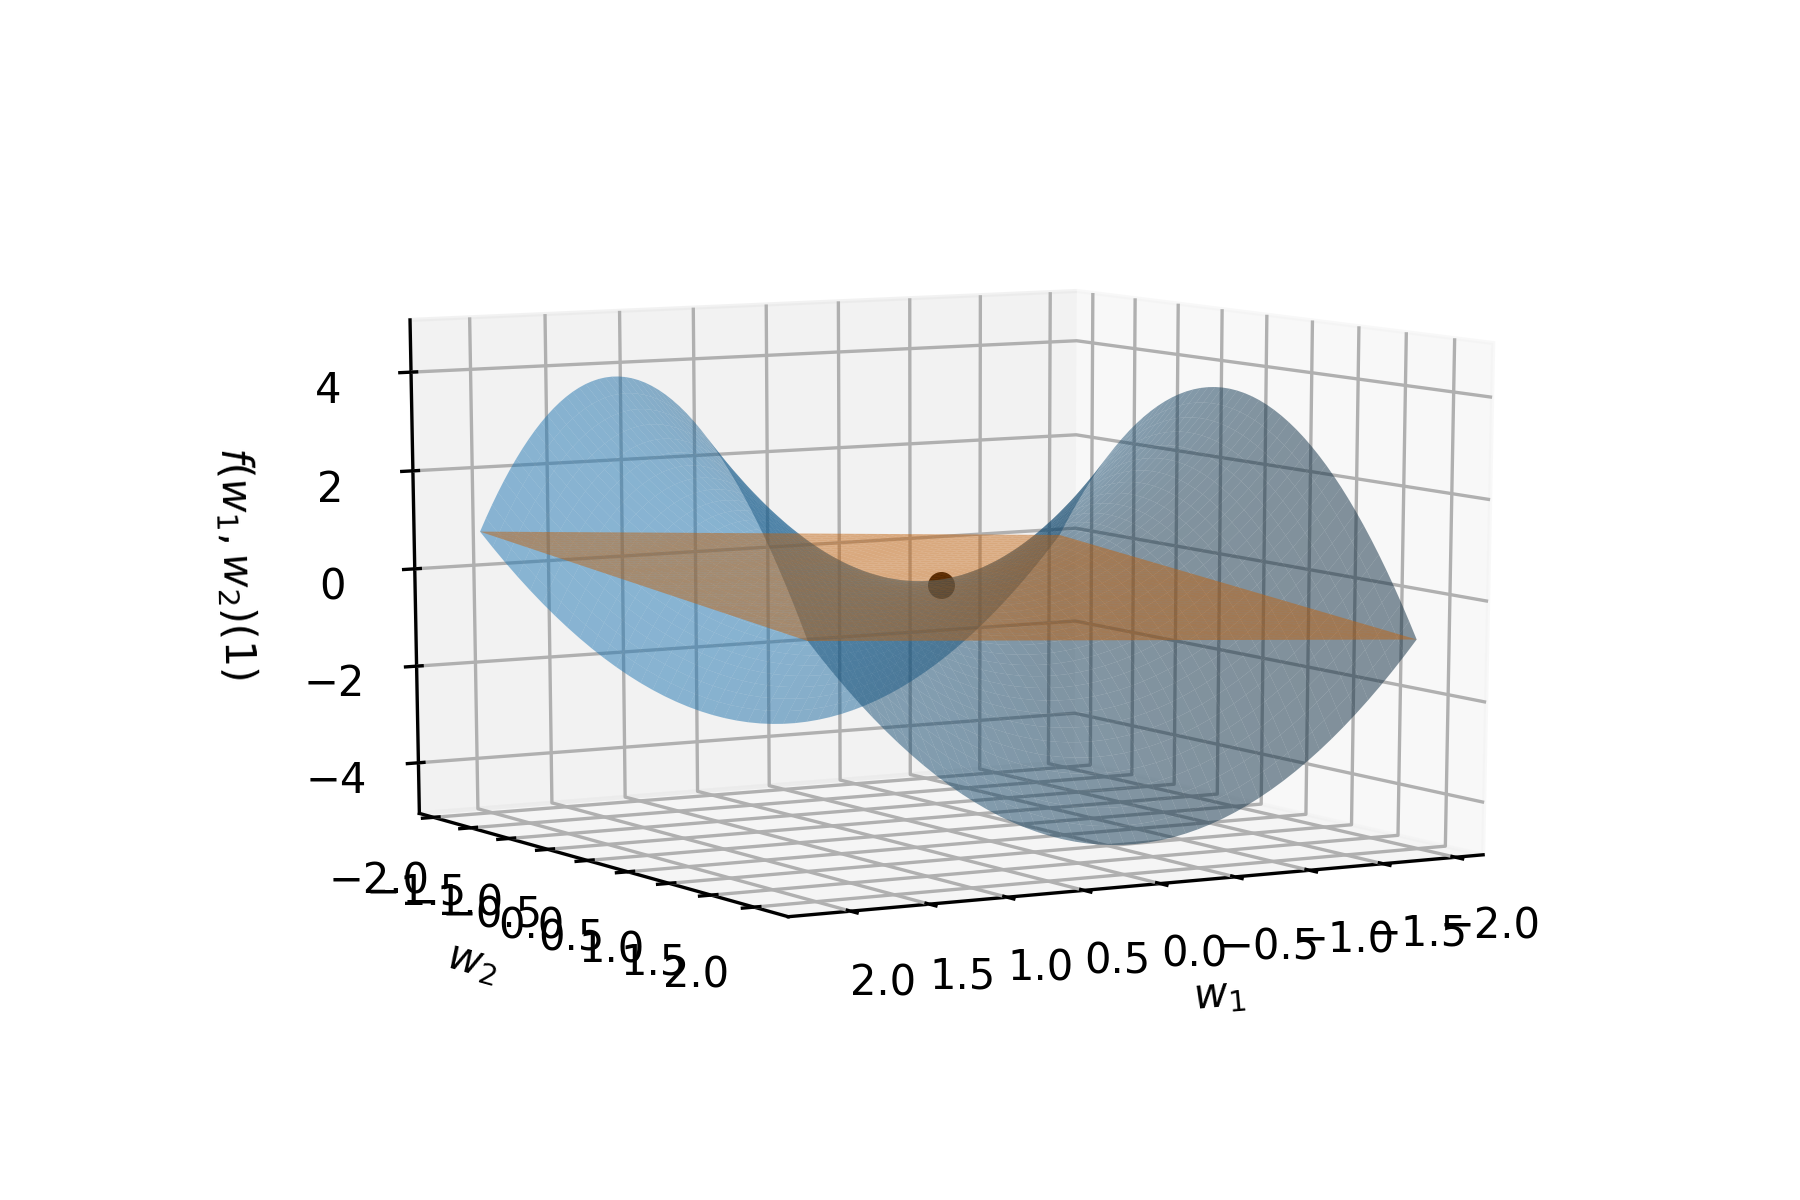
\includegraphics[width=.5\textwidth]{Imgs/Linearized_Model/visualize_linearized_0.1.png}\hfill
    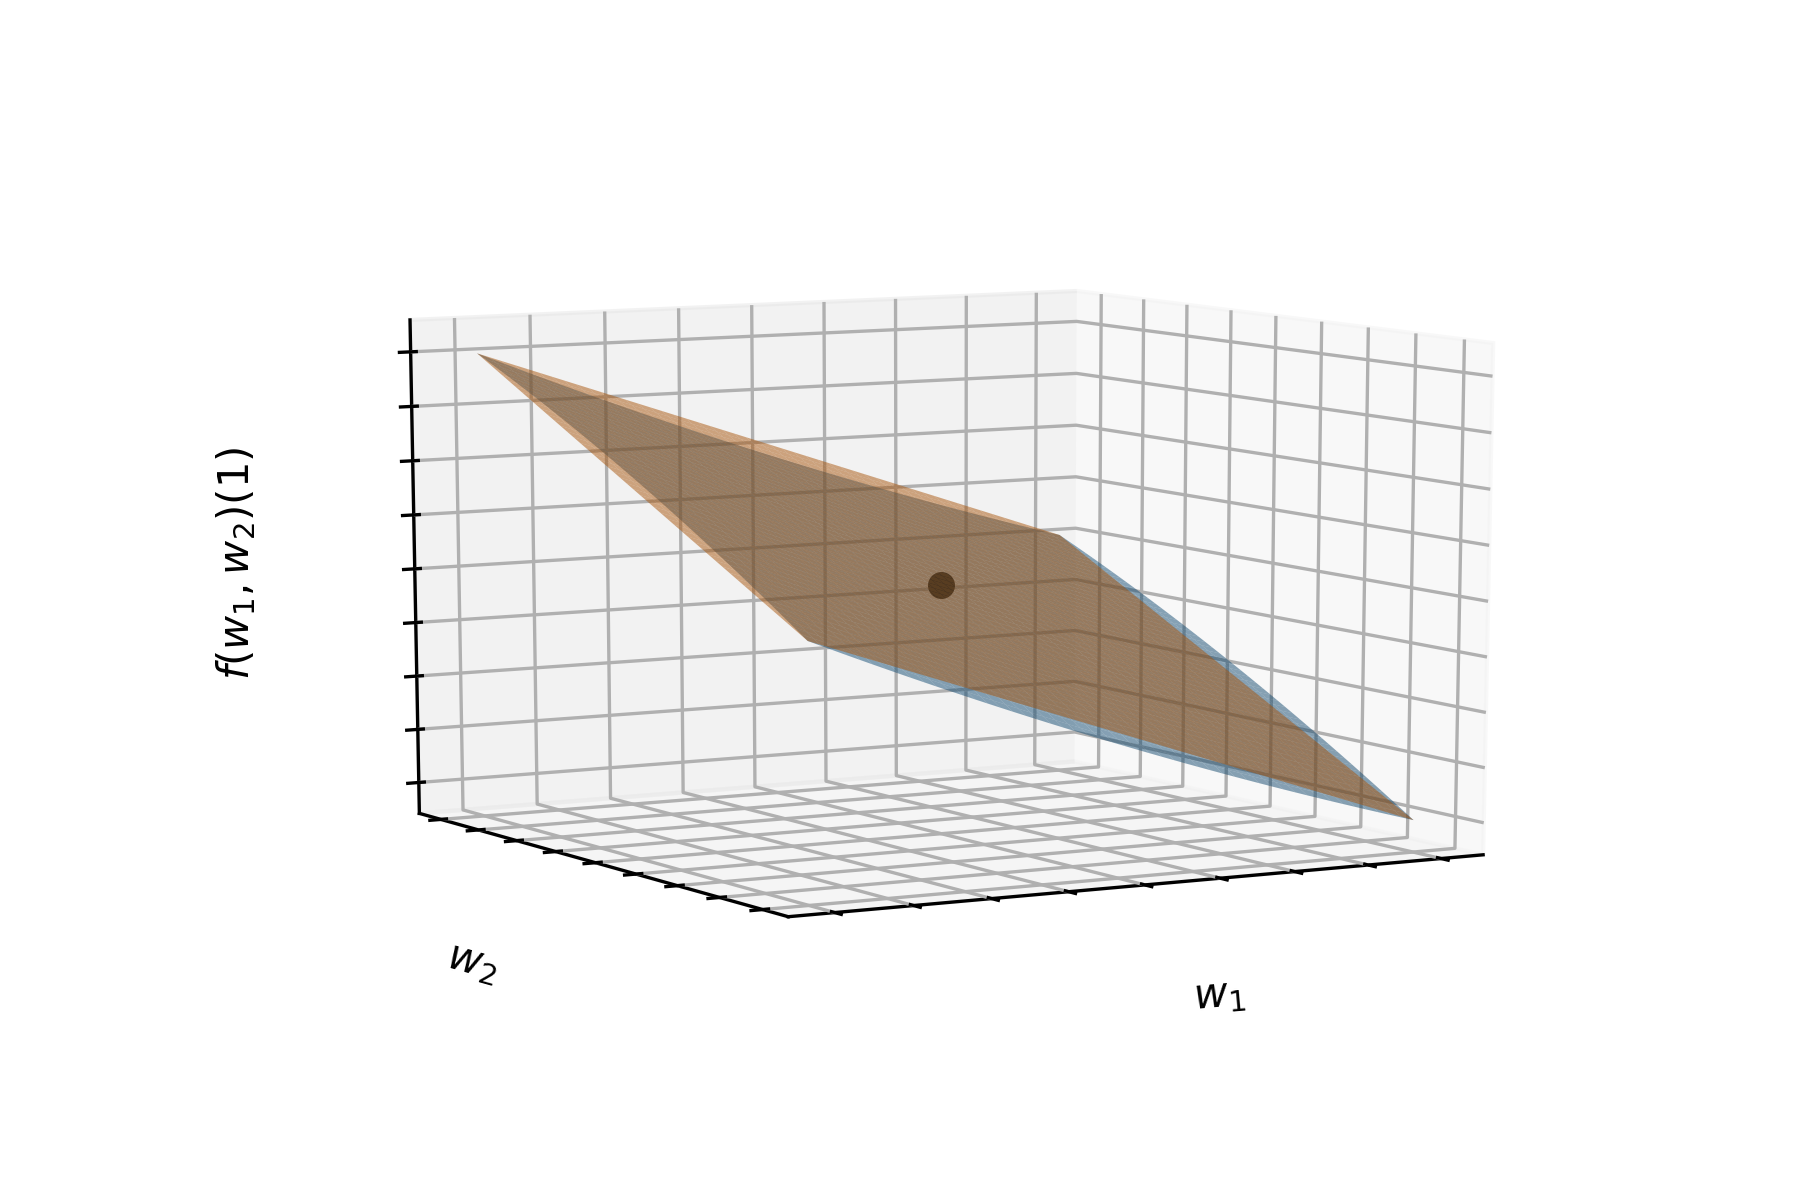
\includegraphics[width=.5\textwidth]{Imgs/Linearized_Model/visualize_linearized_10.png}
    \caption{A neural network with two weights $w_1$, $w_2$ evaluated at the input $1 \in \mathbb{R}$. On the left, notice that the network is highly nonlinear (and nonconvex) in its weights. Conversely, on the right, we see that the function is close to the linearization around its initialization, and so we are approaching the lazy regime.}
\end{figure}

\begin{figure}[H]
\animategraphics[loop, controls, width=\textwidth]{10}{Imgs/Linearized_Model/GIF_imgs/visualize_linearized_}{0}{99}
\caption{Hi foo baz}
\end{figure}


\pagebreak
% References

\bibliographystyle{siam}
\bibliography{References/biblio}

\end{document}